% ------------------------------------------------------------------------------
% TYPO3 CMS 6.2 LTS - What's New (English Version)
% @author Michael Schams <typo3@2013.trash.schams.net>
% @version 1.0.0
%
% ------------------------------------------------------------------------------
% Changelog:
%
% 20 August 2013 - Michael Schams <typo3@2013.trash.schams.net>
%	First initial version
%
% 31 August 2013 - Michael Schams <typo3@2013.trash.schams.net>
%	First two chapters (Introduction and Install Tool) created as proof-of-concept
%
% 01 September 2013 - Michael Schams <typo3@2013.trash.schams.net>
%	Separate chapters into external files
%
% ------------------------------------------------------------------------------

% change the default aspect ratio and frame size
% \documentclass[aspectratio=43]{beamer}
%
% specify vertical top alignment globally by the [t] class option:
% \documentclass[t]{beamer}
%
% for single frames, use the same option locally:
% \begin{frame}[t] ... \end{frame}

\documentclass[t]{beamer}

% suppress navigation bar
\beamertemplatenavigationsymbolsempty

\mode<presentation>
{
	\usetheme{typo3slides}
}

% global variables
\title{TYPO3 CMS 6.2 LTS - What's New}
\subtitle{Summary of the new features, changes and improvements}
\author{(Author)}
\date{\today}

\begin{document}
%\fontsize{15}{18}\selectfont

% select TYPO3 Share font
\sharefont

% ------------------------------------------------------------------------------
% title page
% ------------------------------------------------------------------------------

\begingroup
	\setbeamercolor{normal text}{fg=white,bg=typo3orange}
	\setbeamercolor{title}{fg=white}
	\setbeamercolor{author}{fg=white}
	\setbeamertemplate{footline}[default]
	\begin{frame}
		\titlepage
	\end{frame}
\endgroup

% ------------------------------------------------------------------------------
% table of contents
% ------------------------------------------------------------------------------

% between two frames: use \newpage (not \clearpage!) to force a column break:
% \addtocontents{toc}{\newpage}

\section*{TYPO3 CMS 6.2 LTS - What's New}
\begin{frame}[fragile]
	\frametitle{Chapter Overview}
	\framesubtitle{Chapter Overview}

	\begin{multicols}{2}
		\tableofcontents
	\end{multicols}

\end{frame}

% ------------------------------------------------------------------------------
% Chapter: Introduction
% ------------------------------------------------------------------------------

% ------------------------------------------------------------------------------
% TYPO3 CMS 8.4 - What's New - Chapter "Introduction" (Italian Version)
%
% @author	Michael Schams <schams.net>
% @license	Creative Commons BY-NC-SA 3.0
% @link		http://typo3.org/download/release-notes/whats-new/
% @language	English
% ------------------------------------------------------------------------------
% LTXE-CHAPTER-UID:		7fdf26cc-362160ab-d6c8b905-19722b20
% LTXE-CHAPTER-NAME:	Introduction
% ------------------------------------------------------------------------------

\section{Introduzione}
\begin{frame}[fragile]
	\frametitle{Introduzione}

	\begin{center}\huge{Introduzione}\end{center}
	\begin{center}\huge{\color{typo3darkgrey}\textbf{I fatti in breve}}\end{center}

\end{frame}

% ------------------------------------------------------------------------------
% LTXE-SLIDE-START
% LTXE-SLIDE-UID:		36bbd1e7-b70470c2-e4557331-e851ab9a
% LTXE-SLIDE-ORIGIN:	344cc625-72176049-0721f1aa-0580f11a English
% LTXE-SLIDE-TITLE:		TYPO3 CMS 8.4 - The Facts
% ------------------------------------------------------------------------------
\begin{frame}[fragile]
	\frametitle{Introduzione}
	\framesubtitle{TYPO3 CMS 8.4 - I fatti in breve}

	\begin{itemize}
		\item Data di rilascio: 18 Ottobre 2016
		\item Tipo di rilascio: Sprint Release
		\item Slogan: Fueling
	\end{itemize}

	\begin{figure}
		
\includegraphics[width=0.95\linewidth]{Introduction/typo3cms84-banner.jpg}
	\end{figure}

\end{frame}

% ------------------------------------------------------------------------------
% LTXE-SLIDE-START
% LTXE-SLIDE-UID:		c34db54f-5ce84e64-993b5283-bd1414c5
% LTXE-SLIDE-ORIGIN:	59b04868-09a761b3-0c7ca4c3-ce6e31bb English
% LTXE-SLIDE-TITLE:		System Requirements
% ------------------------------------------------------------------------------
\begin{frame}[fragile]
	\frametitle{Introduzione}
	\framesubtitle{Requisiti di sistema}

	\begin{itemize}
		\item PHP:\tabto{2.2cm}versione 7
		\item MySQL:\tabto{2.2cm}versione da 5.5 a 5.7
		\item Spazio disco:\tabto{2.2cm}min 200 MB
		\item Impostazioni PHP:

			\begin{itemize}
				\item \texttt{memory\_limit} >= 128M
				\item \texttt{max\_execution\_time} >= 240s
				\item \texttt{max\_input\_vars} >= 1500
				\item l'opzione di compilazione \texttt{-}\texttt{-disable-ipv6} \underline{non} deve essere usata
			\end{itemize}

		\item Il Backend richiede Microsoft Internet Explorer 11 o superiore,
			Microsoft Edge, Google Chrome, Firefox, Safari o altro browser recente
			e compatibile

	\end{itemize}

\end{frame}

% ------------------------------------------------------------------------------
% LTXE-SLIDE-START
% LTXE-SLIDE-UID:		6d7a088e-555bc078-1d2027f1-5046d232
% LTXE-SLIDE-ORIGIN:	41f1b51a-6b837f9d-c4aa9584-66f8e47f English
% LTXE-SLIDE-TITLE:		Development And Release Timeline
% ------------------------------------------------------------------------------
\begin{frame}[fragile]
	\frametitle{Introduzione}
	\framesubtitle{Sviluppo e tempi di rilascio}

	\begin{figure}
		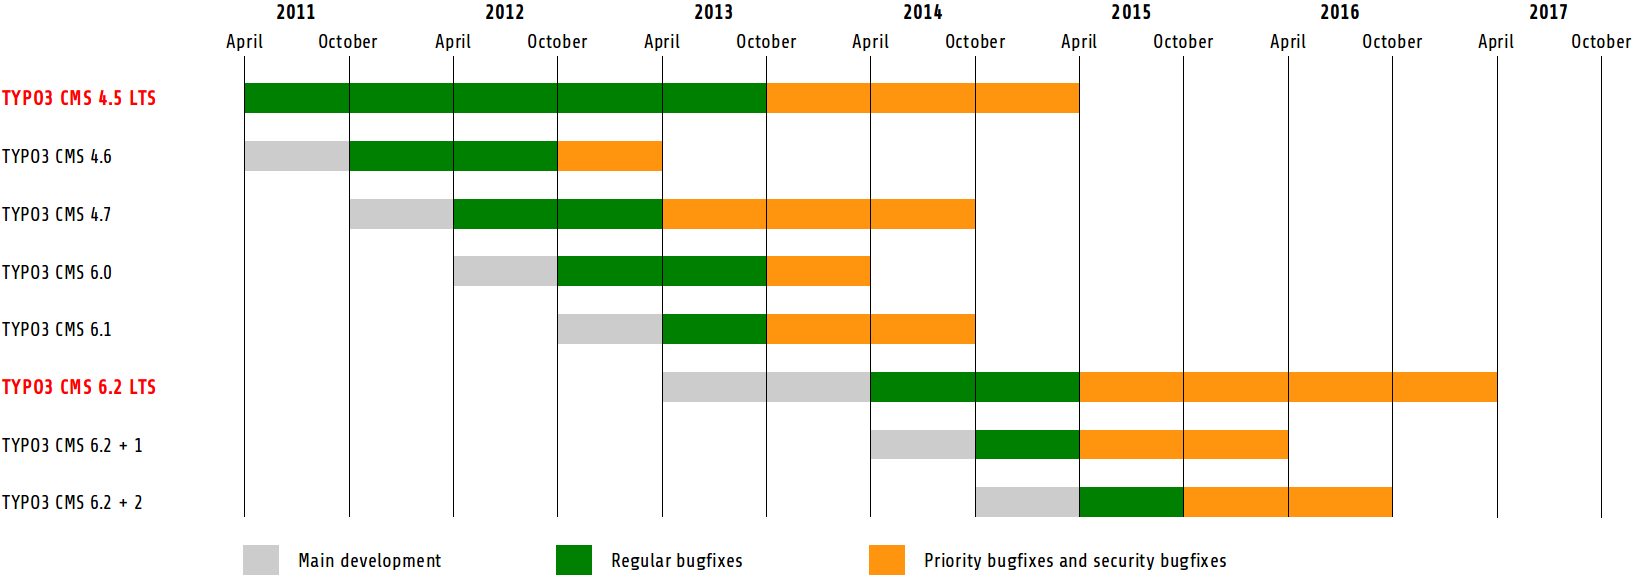
\includegraphics[width=1\linewidth]{Introduction/ReleaseAgenda.png}
	\end{figure}

\end{frame}

% ------------------------------------------------------------------------------
% LTXE-SLIDE-START
% LTXE-SLIDE-UID:		ef57635b-0d6818d0-bc469ed4-3c810ae4
% LTXE-SLIDE-ORIGIN:	f7c981ac-f359aac8-f8799a73-2adc6532 English
% LTXE-SLIDE-TITLE:		TYPO3 CMS Roadmap
% ------------------------------------------------------------------------------
\begin{frame}[fragile]
	\frametitle{Introduzione}
	\framesubtitle{TYPO3 CMS Roadmap}

	Date di rilascio stimate e loro obiettivo principale:

	\begin{itemize}

		\item v8.0 \tabto{1.1cm}22/Mar/2016\tabto{3.4cm}Aggiunta di parti dell'ultimo momento
		\item v8.1 \tabto{1.1cm}03/Mag/2016\tabto{3.4cm}Integrazione cloud
		\item v8.2 \tabto{1.1cm}05/Lug/2016\tabto{3.4cm}Prerequisiti Doctrine
		\item v8.3 \tabto{1.1cm}30/Ago/2016\tabto{3.4cm}Rich Text Editor
		\item
			\begingroup
				\color{typo3orange}
					v8.4 \tabto{1.1cm}18/Ott/2016\tabto{3.4cm}Migrazione Doctrine + Aggiornamenti
			\endgroup
		\item v8.5 \tabto{1.1cm}20/Dic/2016\tabto{3.4cm}Nuovo RTE + Supporto Integrazione
		\item v8.6 \tabto{1.1cm}14/Feb/2017\tabto{3.4cm}\textit{da determinare}
		\item v8.7 \tabto{1.1cm}04/Apr/2017\tabto{3.4cm}Preparazione LTS

	\end{itemize}

	\smaller
		\url{https://typo3.org/typo3-cms/roadmap/}\newline
		\url{https://typo3.org/news/article/kicking-off-typo3-v8-development/}
	\normalsize

\end{frame}

% ------------------------------------------------------------------------------
% LTXE-SLIDE-START
% LTXE-SLIDE-UID:		df4f964f-fa8cb997-19c5170a-4dc9c6b2
% LTXE-SLIDE-ORIGIN:	425f3f15-1178ed7e-f26438f9-a79ad9e9 English
% LTXE-SLIDE-TITLE:		Installation
% ------------------------------------------------------------------------------
\begin{frame}[fragile]
	\frametitle{Introduzione}
	\framesubtitle{Installazione}

	\begin{itemize}
		\item Procedura ufficiale di installazione su Linux/Mac OS X\newline
			(Directory Root ad esempio \texttt{/var/www/site/htdocs}):
		\begin{lstlisting}
			$ cd /var/www/site
			$ wget --content-disposition get.typo3.org/8.4
			$ tar xzf typo3_src-8.4.1.tar.gz
			$ cd htdocs
			$ ln -s ../typo3_src-8.4.1 typo3_src
			$ ln -s typo3_src/index.php
			$ ln -s typo3_src/typo3
			$ touch FIRST_INSTALL
		\end{lstlisting}

		\item Link simbolici in Microsoft Windows:

			\begin{itemize}
				\item Usa \texttt{junction} in Windows XP/2000
				\item Usa \texttt{mklink} in Windows Vista e Windows 7
			\end{itemize}

	\end{itemize}
\end{frame}

% ------------------------------------------------------------------------------
% LTXE-SLIDE-START
% LTXE-SLIDE-UID:		e38ae238-c1d61e71-6406f3e1-8f93121d
% LTXE-SLIDE-ORIGIN:	061ecffe-6aadad2d-6e64a67a-3c50a5cf English
% LTXE-SLIDE-TITLE:		Upgrade to TYPO3 CMS 7
% ------------------------------------------------------------------------------
\begin{frame}[fragile]
	\frametitle{Introduzione}
	\framesubtitle{Aggiornamento a TYPO3 CMS 8.x}

	\begin{itemize}
		\item Aggiornamenti possibili solo da TYPO3 CMS 7.6 LTS
		\item TYPO3 CMS < 7.6 LTS deve essere prima aggiornato a TYPO3 CMS 7.6 LTS
	\end{itemize}

	\begin{itemize}

		\item Istruzioni per l'aggiornamento:\newline
			\smaller\url{http://wiki.typo3.org/Upgrade#Upgrading_to_8.3}\normalsize
		\item Guida ufficiale TYPO3 "TYPO3 Installation and Upgrading":
			\smaller\url{http://docs.typo3.org/typo3cms/InstallationGuide}\normalsize
		\item Approcio generale:
			\begin{itemize}
				\item Verifica i requisiti minimi di sistema \small(PHP, MySQL, etc.)
				\item Verifica \textbf{deprecation\_*.log} nella vecchia istanza TYPO3
				\item Aggiorna tutte le estensioni all'ultima versione
				\item Imposta il nuovo sorgente ed esegui Install Tool -> Upgrade Wizard
				\item Verifica il modulo di startup per gli utenti di backend (opzionale)
			\end{itemize}
	\end{itemize}

\end{frame}

% ------------------------------------------------------------------------------

% ------------------------------------------------------------------------------
% LTXE-SLIDE-START
% LTXE-SLIDE-UID:		5449eaf9-054a9da9-8cccada5-eb6655ca
% LTXE-SLIDE-ORIGIN:	560abc87-898d82d3-b9e35f84-e348c121 English
% LTXE-SLIDE-TITLE:		PHP Version 7
% ------------------------------------------------------------------------------
\begin{frame}[fragile]
	\frametitle{Introduzione}
	\framesubtitle{PHP Version 7}

	\begin{itemize}

		\item PHP 7.0 è un requisito minimo per TYPO3 CMS 8.x
		\item TYPO3 supporterà i successivi rilasci di PHP 7 mano a mano che saranno pubblicati
		\item Questa versione fornisce un significativo incremento delle prestazioni del sistema

		\item Non solo gli editori di backend noteranno un interfaccia più veloce, ma il tempo
			di caricamento di un intera pagina di frontend in cache è inferiore a
			7 millisecondi, che è circa il 40\% più veloce paragonandolo
			allo stesso sito web con PHP versione 5.5

		\item Si sono iniziate ad utilizzare anche le nuove funzioni di questa versione di PHP,
			per esempio i generatori crittografici pseudo-casuali sono già in uso.

	\end{itemize}

\end{frame}

% ------------------------------------------------------------------------------


% ------------------------------------------------------------------------------
% Chapter: Install Tool
% ------------------------------------------------------------------------------

% ------------------------------------------------------------------------------
% TYPO3 CMS 6.2 LTS - What's New - Chapter "Install Tool" (English Version)
%
% @author	Michael Schams <schams.net>
% @license	Creative Commons BY-NC-SA 3.0
% @link		http://typo3.org/download/release-notes/whats-new/
% @language	English
% ------------------------------------------------------------------------------
% Chapter: Install Tool
% ------------------------------------------------------------------------------

\section{Install Tool}
\begin{frame}[fragile]
	\frametitle{Install Tool}

	\begin{center}\huge{Chapter 1:}\end{center}
	\begin{center}\huge{\color{typo3darkgrey}\textbf{The Install Tool}}\end{center}

\end{frame}

% ------------------------------------------------------------------------------
% Installation
% ------------------------------------------------------------------------------

\begin{frame}[fragile]
	\frametitle{Install Tool}
	\framesubtitle{Installation}

	\begin{itemize}
		\item Only \underline{one} package is required for an installation:\newline
				\texttt{typo3\_src-6.2.x.tar.gz} (file size: approx. 20MB)
		\item "Dummy" and "Blank" packages became obsolete
		\item Installation:
			\begin{itemize}
				\item Extract source package into web root directory
				\item Create symbolic links as required
				\item Point web browser to your web root
				\item TYPO3 Installer starts 1-2-3-4-5-steps wizard
			\end{itemize}

	\end{itemize}

\end{frame}

% ------------------------------------------------------------------------------
% Installation
% ------------------------------------------------------------------------------

\begin{frame}[fragile]

	\frametitle{Install Tool}
	\framesubtitle{Installation}

	\begin{itemize}
		\item Installer ensures that all required files and directories are in place
		\item Files required for a custom setup will be created automatically
		\item The following symbolic links \underline{must} exist:

		\begin{itemize}
			\item \texttt{typo3\_src}	\tabto{2cm} (points to TYPO3 source directory)
			\item \texttt{typo3}		\tabto{2cm} (points to directory: \texttt{typo3\_src/typo3})
			\item \texttt{index.php}	\tabto{2cm} (points to file: \texttt{typo3\_src/index.php})
		\end{itemize}

		\item No further files/directories are required to install TYPO3!
		\item Directory \texttt{t3lib} removed
		\item Further details: TYPO3 Installation and Upgrade Guide\newline
			\url{http://docs.typo3.org/typo3cms/InstallationGuide}

	\end{itemize}

\end{frame}

% ------------------------------------------------------------------------------
% Re-Development
% ------------------------------------------------------------------------------

\begin{frame}[fragile]
	\frametitle{Install Tool}
	\framesubtitle{Re-Development}

	\begin{columns}[T]

		\begin{column}{.5\textwidth}
			\begin{itemize}
				\item Re-developed from scratch\newline using Fluid
				\item \underline{First} step tests system environment and reports issues
				\item Reported issues can be fixed\newline (and re-tested) or ignored
				\item Invalid core setup (e.g. no symbolic links as recommended) is reported as an issue, too
			\end{itemize}
		\end{column}

		\begin{column}{.5\textwidth}
			\begin{figure}\vspace*{-0.4cm}
				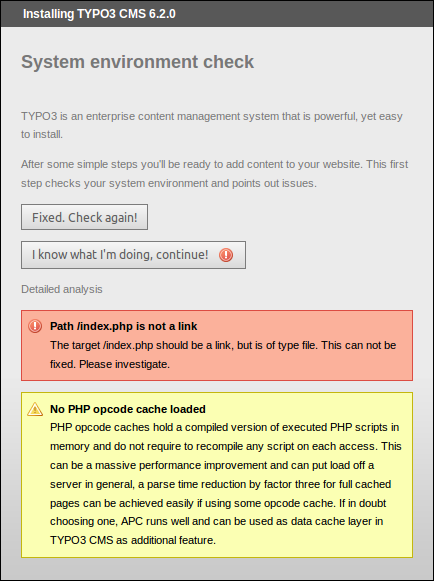
\includegraphics[width=0.8\linewidth]{Images/InstallTool/SystemEnvironmentCheck.png}
			\end{figure}
		\end{column}

	\end{columns}

\end{frame}

% ------------------------------------------------------------------------------
% Re-Development
% ------------------------------------------------------------------------------

\begin{frame}[fragile]
	\frametitle{Install Tool}
	\framesubtitle{Re-Development}

	\begin{columns}[T]

		\begin{column}{.5\textwidth}
			\begin{itemize}
				\item \underline{Second} step allows users to enter database access details
				\item Connection types are selectable
					\begin{itemize}
						\item TCP/IP based connection
						\item Socket based connection
					\end{itemize}
				\item MySQL alternatives are also possible
			\end{itemize}
		\end{column}

		\begin{column}{.5\textwidth}
			\begin{figure}\vspace*{-0.4cm}
				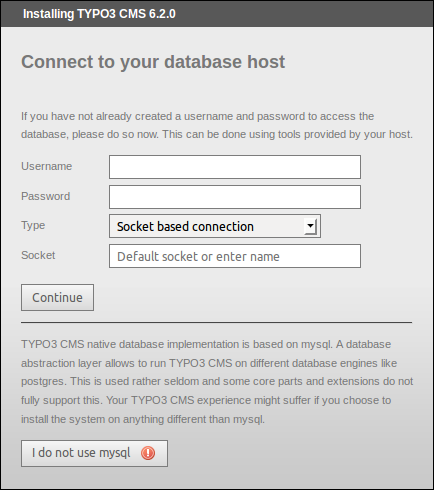
\includegraphics[width=0.8\linewidth]{Images/InstallTool/DatabaseConnectionDetails.png}
			\end{figure}
		\end{column}

	\end{columns}

\end{frame}

% ------------------------------------------------------------------------------
% Re-Development
% ------------------------------------------------------------------------------

\begin{frame}[fragile]
	\frametitle{Install Tool}
	\framesubtitle{Re-Development}

	\begin{columns}[T]

		\begin{column}{.5\textwidth}
			\begin{itemize}
				\item \underline{Third} step allows users to select/create the database\newline
					(as in TYPO3 < 6.2)
				\item \underline{Fourth} step allows users to set a password for the "admin" user\newline (which is also the initial Install Tool password) and a site name
			\end{itemize}
		\end{column}

		\begin{column}{.5\textwidth}
			\begin{figure}\vspace*{-0.4cm}
				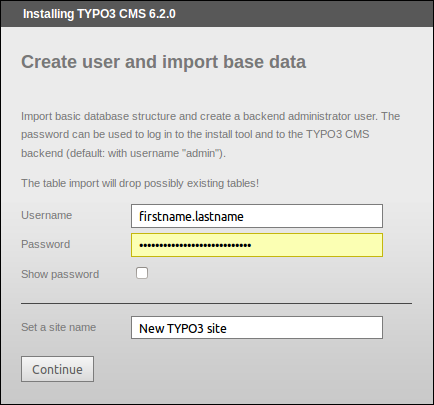
\includegraphics[width=0.8\linewidth]{Images/InstallTool/AdminPasswordAndSiteName.png}
			\end{figure}
		\end{column}

	\end{columns}

\end{frame}

% ------------------------------------------------------------------------------
% Clear All Cache
% ------------------------------------------------------------------------------

\begin{frame}[fragile]
	\frametitle{Install Tool}
	\framesubtitle{Clear All Cache}

	\begin{itemize}
		\item New function under "Important actions" lets users clear all cache
		\item This also works, if cache contains invalid PHP code\newline
			(which possibly locks TYPO3 CMS)
		\item Bypass a not-working TYPO3 instance by accessing the Install Tool directly: \texttt{http://example.com/typo3/install}
	\end{itemize}

	\begin{columns}[T]
		\begin{column}{.3\textwidth}
			\begin{figure}\vspace*{-0.4cm}
				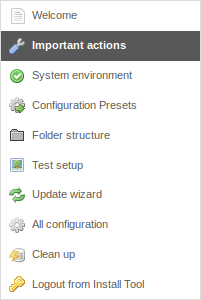
\includegraphics[width=0.7\linewidth]{Images/InstallTool/ImportantActions.png}
			\end{figure}
		\end{column}
		\begin{column}{.7\textwidth}
			\begin{figure}\vspace*{-0.4cm}
				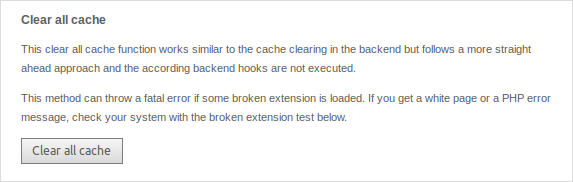
\includegraphics[width=0.9\linewidth]{Images/InstallTool/ClearAllCache.png}
			\end{figure}
		\end{column}
	\end{columns}

\end{frame}

% ------------------------------------------------------------------------------
% Clear All Cache
% ------------------------------------------------------------------------------

\begin{frame}[fragile]
	\frametitle{Install Tool}
	\framesubtitle{Clear All Cache}

	Sequence of actions when executing "Clear all cache":

	\begin{enumerate}
		\item Content of directory \texttt{typo3temp/Cache} is deleted
		\item Database tables \texttt{cf\_*} are emptied
		\item Files \texttt{ext\_localconf.php} and \texttt{ext\_tables.php}\newline
			are loaded from extensions
		\item \texttt{flushCaches()} are executed
	\end{enumerate}

\end{frame}

% ------------------------------------------------------------------------------
% Check For Broken Extensions
% ------------------------------------------------------------------------------

\begin{frame}[fragile]
	\frametitle{Install Tool}
	\framesubtitle{Check For Broken Extensions}

	\begin{itemize}
		\item New function under "Important actions" lets users check,\newline
			if extensions can be loaded without breaking the system
		\item Very useful for an update from TYPO3 4.5 to 6.2
	\end{itemize}

	\begin{columns}[T]
		\begin{column}{.3\textwidth}
			\begin{figure}\vspace*{-0.4cm}
				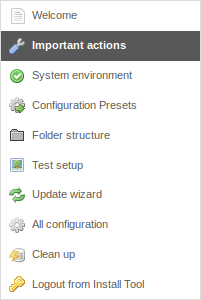
\includegraphics[width=0.7\linewidth]{Images/InstallTool/ImportantActions.png}
			\end{figure}
		\end{column}
		\begin{column}{.7\textwidth}
			\begin{figure}\vspace*{-0.4cm}
				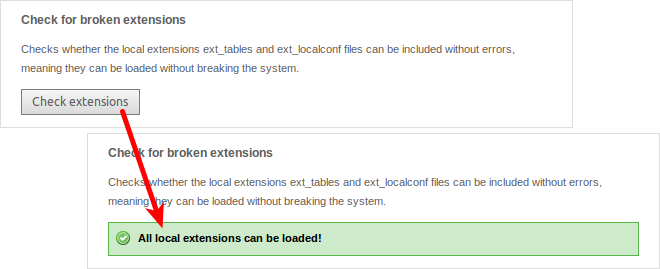
\includegraphics[width=1\linewidth]{Images/InstallTool/CheckForBrokenExtensions.png}
			\end{figure}
		\end{column}
	\end{columns}

\end{frame}

% ------------------------------------------------------------------------------
% Increased Security: Salted Passwords
% ------------------------------------------------------------------------------

\begin{frame}[fragile]
	\frametitle{Install Tool}
	\framesubtitle{Salted Passwords}

	\begin{itemize}
		\item When creating new backend administrator user via Install Tool,\newline
			a \textbf{salted} password is used\newline
			\smaller(requires installed, loaded and configured EXT:saltedpasswords)\normalsize
		\item Install Tool password is a \textbf{salted} password as well\newline
			\smaller(existing MD5 hashes are converted automatically at first login)\normalsize
	\end{itemize}

	\begin{columns}[T]
		\begin{column}{.3\textwidth}
			\begin{figure}\vspace*{-0.4cm}
				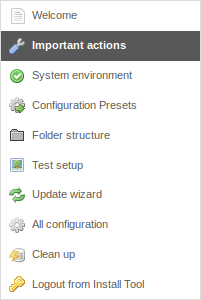
\includegraphics[width=0.7\linewidth]{Images/InstallTool/ImportantActions.png}
			\end{figure}
		\end{column}
		\begin{column}{.7\textwidth}
			\begin{figure}\vspace*{-0.4cm}
				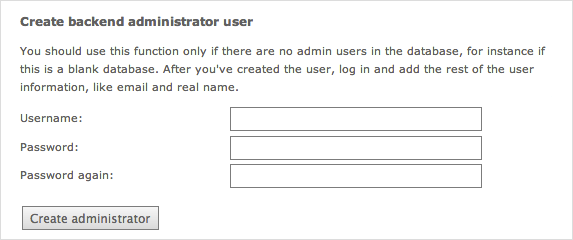
\includegraphics[width=0.9\linewidth]{Images/InstallTool/SaltedPasswords.png}
			\end{figure}
		\end{column}
	\end{columns}

\end{frame}

% ------------------------------------------------------------------------------
% Application Context
% ------------------------------------------------------------------------------

\begin{frame}[fragile]
	\frametitle{Install Tool}
	\framesubtitle{Application Context (1)}

	\begin{itemize}
		\item TYPO3 >= 6.2 takes \textbf{Application Context} into account\newline
			\smaller(known from TYPO3 Flow)\normalsize
		\item Environment variable \texttt{TYPO3\_CONTEXT} sets the context\newline
			\smaller(default: \texttt{Production}, sub-context such as \texttt{Production/Staging} possible)\normalsize

			\begin{lstlisting}
				# File: .htaccess
				# Rules to set Application Context based on hostname:

				RewriteCond %{HTTP_HOST} ^dev\.example\.com$
				RewriteRule (.*) $1 [E=TYPO3_CONTEXT:Development]

				RewriteCond %{HTTP_HOST} ^www\.example\.com$
				RewriteRule (.*) $1 [E=TYPO3_CONTEXT:Production]

				# Sets an environment variable, which is then available to TYPO3 CMS:
				SetEnv TYPO3_CONTEXT Production
			\end{lstlisting}

	\end{itemize}

\end{frame}

% ------------------------------------------------------------------------------
% Presets of TYPO3_CONF_VAR Settings
% ------------------------------------------------------------------------------

\begin{frame}[fragile]
	\frametitle{Install Tool}
	\framesubtitle{Presets of TYPO3\_CONF\_VAR Settings}

	\begin{columns}[T]
		\begin{column}{.5\textwidth}

			\begin{itemize}
				\item Certain \texttt{TYPO3\_CONF\_VAR} settings can be configured in Install Tool
				\item Settings such as debug output, deprecation log, devIPmask and other system logs and log levels
				\item Build-in contexts: "Production" and "Development"\newline
					(custom configuration is also possible)
			\end{itemize}

		\end{column}
		\begin{column}{.5\textwidth}

			\begin{figure}\vspace*{-0.4cm}
				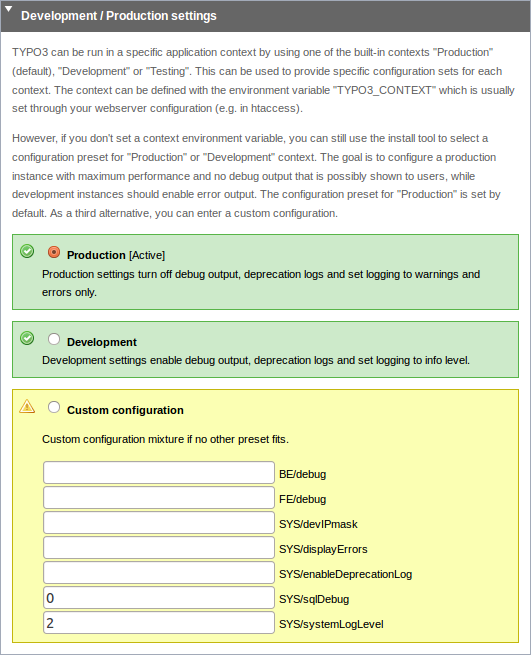
\includegraphics[width=0.8\linewidth]{Images/InstallTool/PresetsOfSettings.png}
			\end{figure}

		\end{column}
	\end{columns}

\end{frame}

% ------------------------------------------------------------------------------
% Improved Usability
% ------------------------------------------------------------------------------

\begin{frame}[fragile]
	\frametitle{Install Tool}
	\framesubtitle{Improved Usability}

	\begin{columns}[T]
		\begin{column}{.5\textwidth}

			\begin{itemize}
				\item Fixed position of menu left-\newline
					hand-side when scrolling
					\begingroup\color{typo3red}\textbf{(1)}\endgroup
				\item Fixed position of button "Write configuration" at the bottom
					\begingroup\color{typo3red}\textbf{(2)}\endgroup
				\item Entries in "All Configuration" are grouped (unfold a section by click on headline) and sorted
					\begingroup\color{typo3red}\textbf{(3)}\endgroup
			\end{itemize}

		\end{column}
		\begin{column}{.5\textwidth}

			\begin{figure}\vspace*{-0.4cm}
				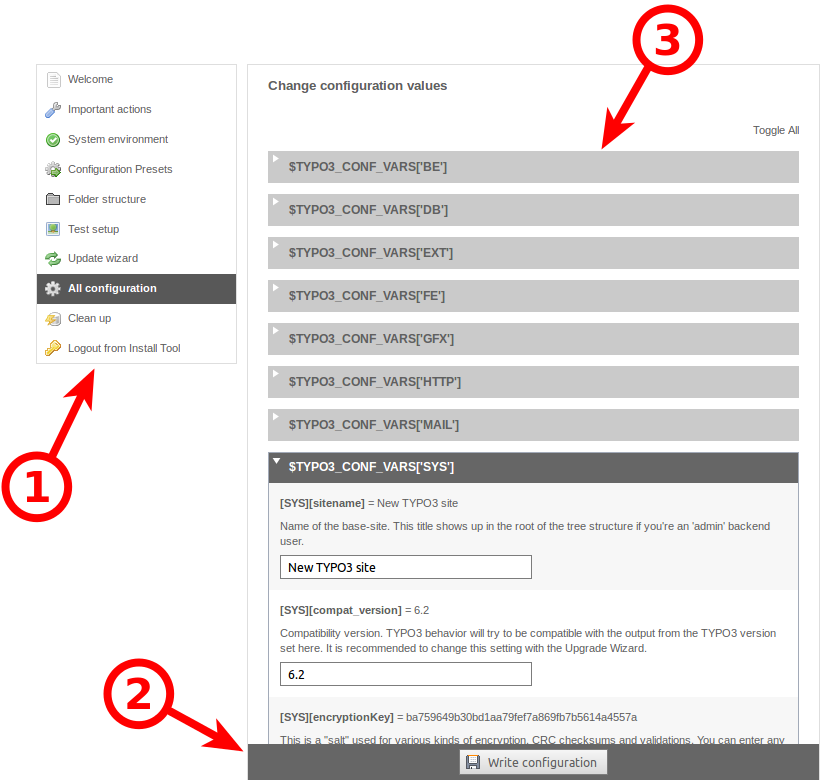
\includegraphics[width=0.8\linewidth]{Images/InstallTool/ImprovedUsability.png}
			\end{figure}

		\end{column}
	\end{columns}

\end{frame}

% ------------------------------------------------------------------------------
% Human-Friendly Error Codes
% ------------------------------------------------------------------------------

\begin{frame}[fragile]
	\frametitle{Install Tool}
	\framesubtitle{Human-Friendly Error Codes}

	\begin{itemize}
		\item Meaningful keywords can be used for the following options:\newline
			(TYPO3 < 6.2: numeric values only)
	\end{itemize}

	\begin{columns}[T]
		\begin{column}{.4\textwidth}
			\advance\leftskip+0.8cm

			\smaller
				\texttt{[SYS][errorHandlerErrors]}\newline
				\texttt{[SYS][exceptionalErrors]}\newline
				\texttt{[SYS][syslogErrorReporting]}\newline
				\texttt{[SYS][belogErrorReporting]}\newline
			\normalsize

		\end{column}
		\begin{column}{.6\textwidth}

			\begin{figure}\vspace*{-0.4cm}
				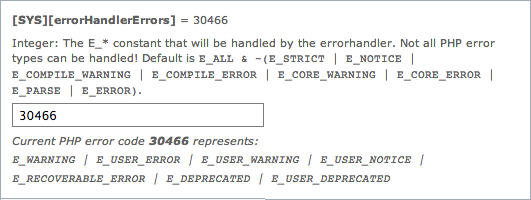
\includegraphics[width=0.9\linewidth]{Images/InstallTool/HumanFriendlyErrorCodes.png}
			\end{figure}

		\end{column}
	\end{columns}

	\vspace{0.2cm}

	\begin{itemize}
		\item An Extbase ViewHelper \textbf{format.phpErrorCode} takes care of the conversion to PHP error codes
	\end{itemize}

\end{frame}

% ------------------------------------------------------------------------------
% Errors In Folder Structure
% ------------------------------------------------------------------------------

\begin{frame}[fragile]
	\frametitle{Install Tool}
	\framesubtitle{Errors In Folder Structure}

	\begin{itemize}
		\item Errors under "Folder Structure" are listed as a badge (circled number)
	\end{itemize}

	\begin{figure}
		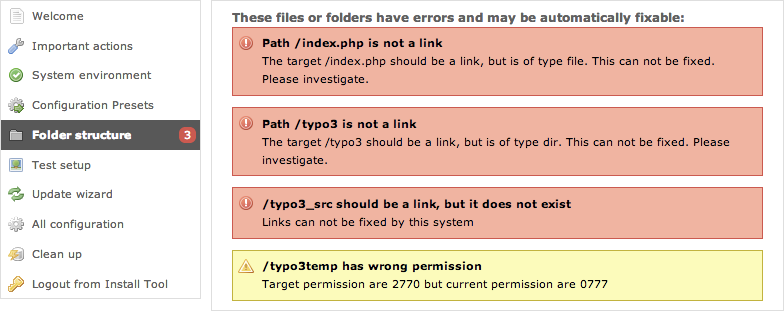
\includegraphics[width=0.95\linewidth]{Images/InstallTool/ErrorsInFolderStructure.png}
	\end{figure}

\end{frame}

% ------------------------------------------------------------------------------
% Core Updates
% ------------------------------------------------------------------------------

\begin{frame}[fragile]
	\frametitle{Install Tool}
	\framesubtitle{Core Updates}

	\begin{itemize}
		\item Update TYPO3 core to its latest minor version with a click of a button 
		\item Environment variable \texttt{TYPO3\_DISABLE\_CORE\_UPDATER=1} disables this feature
	\end{itemize}

	\begin{figure}
		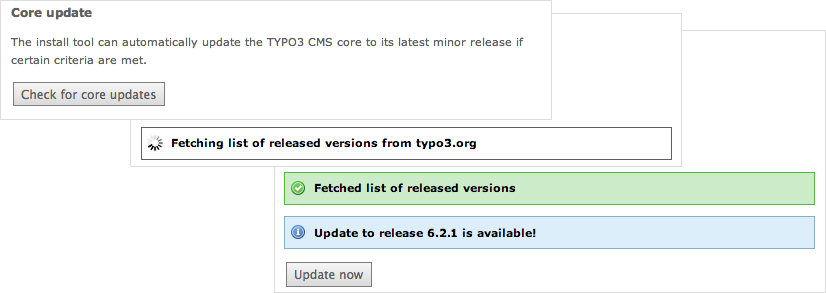
\includegraphics[width=0.95\linewidth]{Images/InstallTool/CoreUpdate.png}
	\end{figure}

\end{frame}

% ------------------------------------------------------------------------------
% Miscellaneous
% ------------------------------------------------------------------------------

\begin{frame}[fragile]
	\frametitle{Install Tool}
	\framesubtitle{Miscellaneous}

	\begin{itemize}
		\item All forms are CSRF (\textit{cross-site request forgery}) protected
		\item Install Tool uses a simplified Fluid Standalone View
		\item Only essential TYPO3 functions are loaded\newline
			(corrupt \texttt{ext\_localconf.php} or \texttt{ext\_tables.php} of extensions can not break the Install Tool any more)
		\item New starting point:	\tabto{3.2cm} \texttt{typo3/sysext/install/Start/Install.php}\newline
			Before:					\tabto{3.2cm} \texttt{typo3/install/index.php}\newline
									\tabto{3.2cm} (redirect from old to new URL exists)
		\item Deactivated cache ensures that Install Tool remains usable, even if cache contains invalid PHP code
	\end{itemize}

\end{frame}

% ------------------------------------------------------------------------------
% Miscellaneous
% ------------------------------------------------------------------------------

\begin{frame}[fragile]
	\frametitle{Install Tool}
	\framesubtitle{Miscellaneous}

	\begin{itemize}
		\item Check if PHP option \texttt{xdebug.max\_nesting\_level} shows a value of 250 or higher (default value "100" possibly causes problems)
		\item "Relaxed permission check":

			\small
				If the web root folder does not have correct permissions set (e.g. "2770"),
				and this issue can not be fixed, e.g. because the directory does not belong
				to the system user who runs the Install Tool, the first step of the installation
				breaks.
				The option "targetPermissionRelaxed" lowers the severity if permissions are not
				ideal and allows for continuing installation as long as required sub folders can
				be created.
			\normalsize

	\end{itemize}

\end{frame}

% ------------------------------------------------------------------------------
% Miscellaneous
% ------------------------------------------------------------------------------

\begin{frame}[fragile]
	\frametitle{Install Tool}
	\framesubtitle{Miscellaneous}

	\begin{itemize}
		\item Removed options (keys) from Install Tool\newline
			\small(and therefore from file \texttt{LocalConfiguration.php}, too):\normalsize
	\end{itemize}

	\begin{columns}[T]
		\begin{column}{.5\textwidth}
			\advance\leftskip+0.8cm
			\smaller
				\texttt{BE/loginLabels}\newline
				\texttt{BE/loginNews}\newline
				\texttt{BE/useOnContextMenuHandler}\newline
				\texttt{EXT/em\_mirrorListURL}\newline
				\texttt{EXT/em\_wsdlURL}\newline
				\texttt{EXT/extList}\newline
				\texttt{EXT/extList\_FE}\newline
				\texttt{EXT/noEdit}\newline
			\normalsize
		\end{column}
		\begin{column}{.5\textwidth}
			\smaller
				\texttt{FE/defaultTypoScript\_editorcfg}\newline
				\texttt{FE/simulateStaticDocuments}\newline
				\texttt{GFX/noIconProc}\newline
				\texttt{GFX/TTFLocaleConv}\newline
				\texttt{SYS/additionalAllowedClassPrefixes}\newline
				\texttt{SYS/caching/cacheBackends}\newline
				\texttt{SYS/caching/cacheFrontends}\newline
				\texttt{SYS/extCache}\newline
				\texttt{SYS/T3instID}\newline
			\normalsize
		\end{column}

	\end{columns}

\end{frame}

% ------------------------------------------------------------------------------



% ------------------------------------------------------------------------------
% Chapter: Test Chapter
% ------------------------------------------------------------------------------

\section{Test Chapter}
\begin{frame}[fragile]
	\frametitle{Test Chapter}

	\begin{center}\huge{Chapter 2:}\end{center}
	\begin{center}\huge{\color{typo3darkgrey}\textbf{The Test Chapter}}\end{center}

\end{frame}

% ------------------------------------------------------------------------------
% Standard Slide
% ------------------------------------------------------------------------------

\begin{frame}
	\frametitle{Test Chapter}
	\framesubtitle{Font Styles}

	\begin{itemize}
		\item \emph{emphasis}
		\item \textsf{Sans}
		\item \texttt{teletypefont}
		\item \textit{italic}
		\item \underline{underline}
		\item \uppercase{uppercase}
		\item \textbf{bold}
		\item \alert{alert}
		\item
			\begingroup
				\color{typo3orange}
				typo3orange
			\endgroup

	\end{itemize}

\end{frame}

% ------------------------------------------------------------------------------
% Standard Slide
% ------------------------------------------------------------------------------

\begin{frame}
	\frametitle{Test Chapter}
	\framesubtitle{Links}

	\begin{itemize}
		\item Item
		\item Item with link: \url{http://typo3.org}
		\item Item with \href{http://typo3.org}{link label}

		\item First level
		\begin{itemize}
			\item Second level
			\begin{itemize}
				\item Third level
			\end{itemize}
		\end{itemize}

	\end{itemize}

\end{frame}

% ------------------------------------------------------------------------------
% Standard Slide
% ------------------------------------------------------------------------------

\begin{frame}
	\frametitle{Test Chapter}
	\framesubtitle{Item List}

	\begin{itemize}
		\item Item 1
		\item Item 2
		\item Item 3
		\item Item 4
		\item Item 5
		\item Item 6
		\item Item 7
		\item Item 8
		\item Item 9
		\item Item 10
		\item Item 11
		\item Item 12
	\end{itemize}

\end{frame}

% ------------------------------------------------------------------------------

% an empty frame to enforce entries in the table of contents
% *TODO* to be removed later

\section{Empty Frame}
\begin{frame}
\end{frame}

\end{document}

